\capitulo{1}{Introducción}

Una endodoncia \cite{soares2002endodoncia} se realiza cuando se infecta o se inflama la parte interna del diente, denominada pulpa, y que contiene los vasos sanguíneos y el nervio del diente. Dicho proceso, busca eliminar la pulpa de forma parcial o total, para salvar el diente en su totalidad, y rellenarlo de un material inerte.

La endodoncia es necesaria, ya que al encontrarse la inflamación en el interior de un diente y al no ser un tejido elástico, puede causar un gran dolor.

Los cuatro factores más comunes que dan lugar a una posible endodoncia son los siguientes \cite{causas2020}:
\begin{itemize}
    \item \textbf{Caries profundas:} si una caries no se trata de forma correcta y a tiempo, puede acabar llegando a la pulpa del diente, dando lugar a una inflamación de la zona.
    \item \textbf{Traumatismos:} los golpes en los dientes pueden dar lugar a roturas de los tejidos internos del diente, produciendo en la mayoría de los casos una infección de la pulpa.
    \item \textbf{Bruxismo:} se produce con el choque de unos dientes con otros haciendo que se desgaste el diente hasta llegar a la pulpa.
    \item \textbf{Periodontitis:} es una enfermedad que ataca al tejido bucal y que puede llegar al interior del diente en caso de que no se trate a tiempo, produciendo una inflamación de la pulpa.
\end{itemize}

Los odontólogos, antes de realizar la endodoncia, necesitan conocer la longitud del diente implicado. Para dicho proceso, los odontólogos llevan a cabo una radiografía de la zona involucrada y posteriormente miden sobre ella la longitud del diente (Figura \ref{f:endo1}). 

A continuación, introducen una varilla en el diente con un tope de longitud menor o igual a la obtenida de la radiografía (Figura \ref{f:endo2}). De nuevo, se hace una radiografía del diente con la varilla y se calcula lo que falta al instrumento para llegar al final del diente (Figura \ref{f:endo3}). Finalmente, se suman la longitud de la varilla introducida y la parte que faltaba hasta llegar al final del diente (Figura \ref{f:endo4}).

\begin{figure}[h]
 \centering
  \subfloat[Medición sobre la radiografía]{
   \label{f:endo1}
    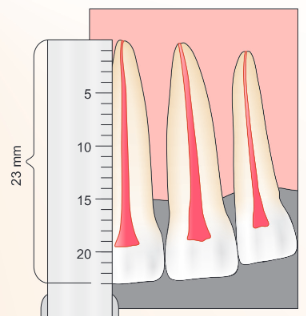
\includegraphics[width=0.4\textwidth]{img/Endodoncia1.PNG}}
  \subfloat[Ajuste de la varilla]{
   \label{f:endo2}
    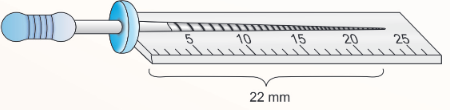
\includegraphics[width=0.4\textwidth]{img/Endodoncia2.PNG}}
  \newline
  \subfloat[Radiografía con la varilla]{
   \label{f:endo3}
    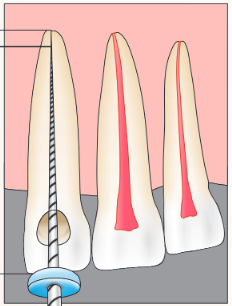
\includegraphics[width=0.35\textwidth]{img/Endodoncia3.PNG}}
  \subfloat[Estimación final del tamaño del diente]{
   \label{f:endo4}
    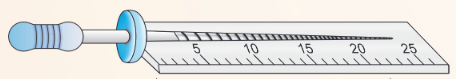
\includegraphics[width=0.4\textwidth]{img/Endodoncia4.PNG}}
 \caption{Ejemplo Proceso Medición Diente \cite{lsm2020proceso}}
 \label{f:endo}
\end{figure}

Todo este proceso es manual. Por tanto, la probabilidad de cometer errores en el proceso de cálculo de medidas es bastante alta. Esta es una de las causas que hacen que el uso del \emph{deep learning} en la rama de la odontología permita obtener una mayor precisión, además de ser una herramienta de apoyo que facilita el trabajo de los odontólogos. Algunas de las principales tareas que puede realizar son \cite{kang2020application}:
\begin{itemize}
    \item Detección y segmentación de dientes y nervios.
    \item Detección de enfermedades.
    \item Fabricación de prótesis.
    \item Detección de implantes junto con la predicción de éxito del mismo.
\end{itemize}

Este proyecto busca automatizar el proceso de medición de la longitud del diente, de forma que a través de una radiografía se pueda dar un valor preciso de su longitud, evitando así cualquier error humano durante la medición y facilitando al odontólogo todo el proceso de medición del diente.

Para ello, el proyecto trabajará con técnicas del \emph{deep learning} para ser capaz de segmentar dientes y nervios en las radiografías, y gracias a esta segmentación poder calcular la longitud del diente deseado.

\section{Estructura}
Este trabajo está formado por dos documentos principales: la Memoria y el Anexo. Cuya estructura es la siguiente:

\subsection{Memoria}
La memoria está formada por los siguientes puntos:
\begin{enumerate}
    \item \textbf{Introducción:} puesta en contexto del problema al que se va enfrentar el proyecto. También se incluyen los documentos adjuntos junto con la estructura de cada uno de ellos.
    \item \textbf{Objetivos del Proyecto:} descripción de los objetivos generales y técnicos.
    \item \textbf{Conceptos Teóricos:} explicación de los diferentes conceptos teóricos que necesitan ser comprendidos para entender todo el proyecto.
    \item \textbf{Técnicas y Herramientas:} contiene una breve descripción de todas las herramientas usadas y metodología seguida a lo largo de todo el proyecto.
    \item \textbf{Aspectos Relevantes del Desarrollo del Proyecto:} exposición de aquellos aspectos más importantes surgidos durante el desarrollo.
    \item \textbf{Trabajos Relacionados:} selección de algunos trabajos que tienen una cierta conexión con la endodoncia y el \emph{deep learning}.
    \item \textbf{Conclusiones y Líneas de Trabajo Futuras:} contiene las conclusiones finales junto con las posibles mejoras o actualizaciones que podría tener la aplicación en el futuro.
\end{enumerate}

\subsection{Anexo}
El anexo está formado por cinco apéndices:
\begin{enumerate}
    \item \textbf{Plan de Proyecto:} contiene el desarrollo que se ha llevado mediante las destinas tareas que se marcaban en cada \emph{sprint}. Además, contiene el estudio de viabilidad del proyecto, a través del análisis de la viabilidad económica y legal.
    \item \textbf{Especificación de Requisitos:} contiene los objetivos generales, los requisitos funcionales y los distintos casos de uso.
    \item \textbf{Especificación de Diseño:} se centra en los diseños de datos, procedimental y arquitectónico.
    \item \textbf{Documentación Técnica de Programación:} contiene la estructura de directorios, manual del programador, ejecución del proyecto y las pruebas del sistema.
    \item \textbf{Documentación de Usuario:} describe los requisitos de usuario, la instalación y el manual de usuario.
\end{enumerate}
